\chapter{Progettazione Concettuale}

\section{Premesse alla lettura dei diagrammi}

\subsubsection{Modelli Utilizzati}

Procediamo alla modellizzazione del mini-mondo, partendo dalla progettazione concettuale.

Questa fase di progettazione è stata svolta utilizzando, oltre che il modello \textbf{UML} nella forma di un \textbf{Class Diagram}, anche il modello \textbf{EER}, ovvero \textbf{Enhanced Entity Relationship}, per cogliere meglio aspetti del dominio che un modello \textbf{ER} classico non avrebbe potuto cogliere, come ad esempio \textbf{generalizzazioni e specializzazioni}.

\subsubsection{Precisazioni sui Diagrammi}

Per migliorare la leggibilità dei diagrammi, si è deciso di specificare le \textbf{molteplicità} degli attributi esclusivamente per sottolineare la possibilità di essere valorizzato a \textbf{NULL}. In tali casi si è utilizzata la molteplicità \textbf{[\(0..1\)]} esclusivamente per gli attributi di tipo \textbf{Bool}, mentre \textbf{[\(0..*\)]} per gli altri.

\bigskip

\begin{note}[Leggibilità dei Diagrammi]
  In caso di problemi di leggibilità dei diagrammi, sono disponibili le versioni originali nella pagina GitHub del progetto: \href{https://github.com/RiccardoElena/UninaDelivery/blob/develop/db/docs/sources/ER_Diagram.pdf}{\textit{\underline{ER Diagram}}} e \href{https://github.com/RiccardoElena/UninaDelivery/blob/develop/db/docs/sources/UML_Class_Diagram.pdf}{\textit{\underline{UML Class Diagram}}}.
\end{note}

\newpage

% TODO: @zGenny UML needs to be polished (line overlappping and 'create' missing 's')
% TODO: @zGenny ER needs to be completed (missing attributes to zone and address, business mail is not PK)

\section{Enhanced Entity Relationship Diagram}
\begin{center}
  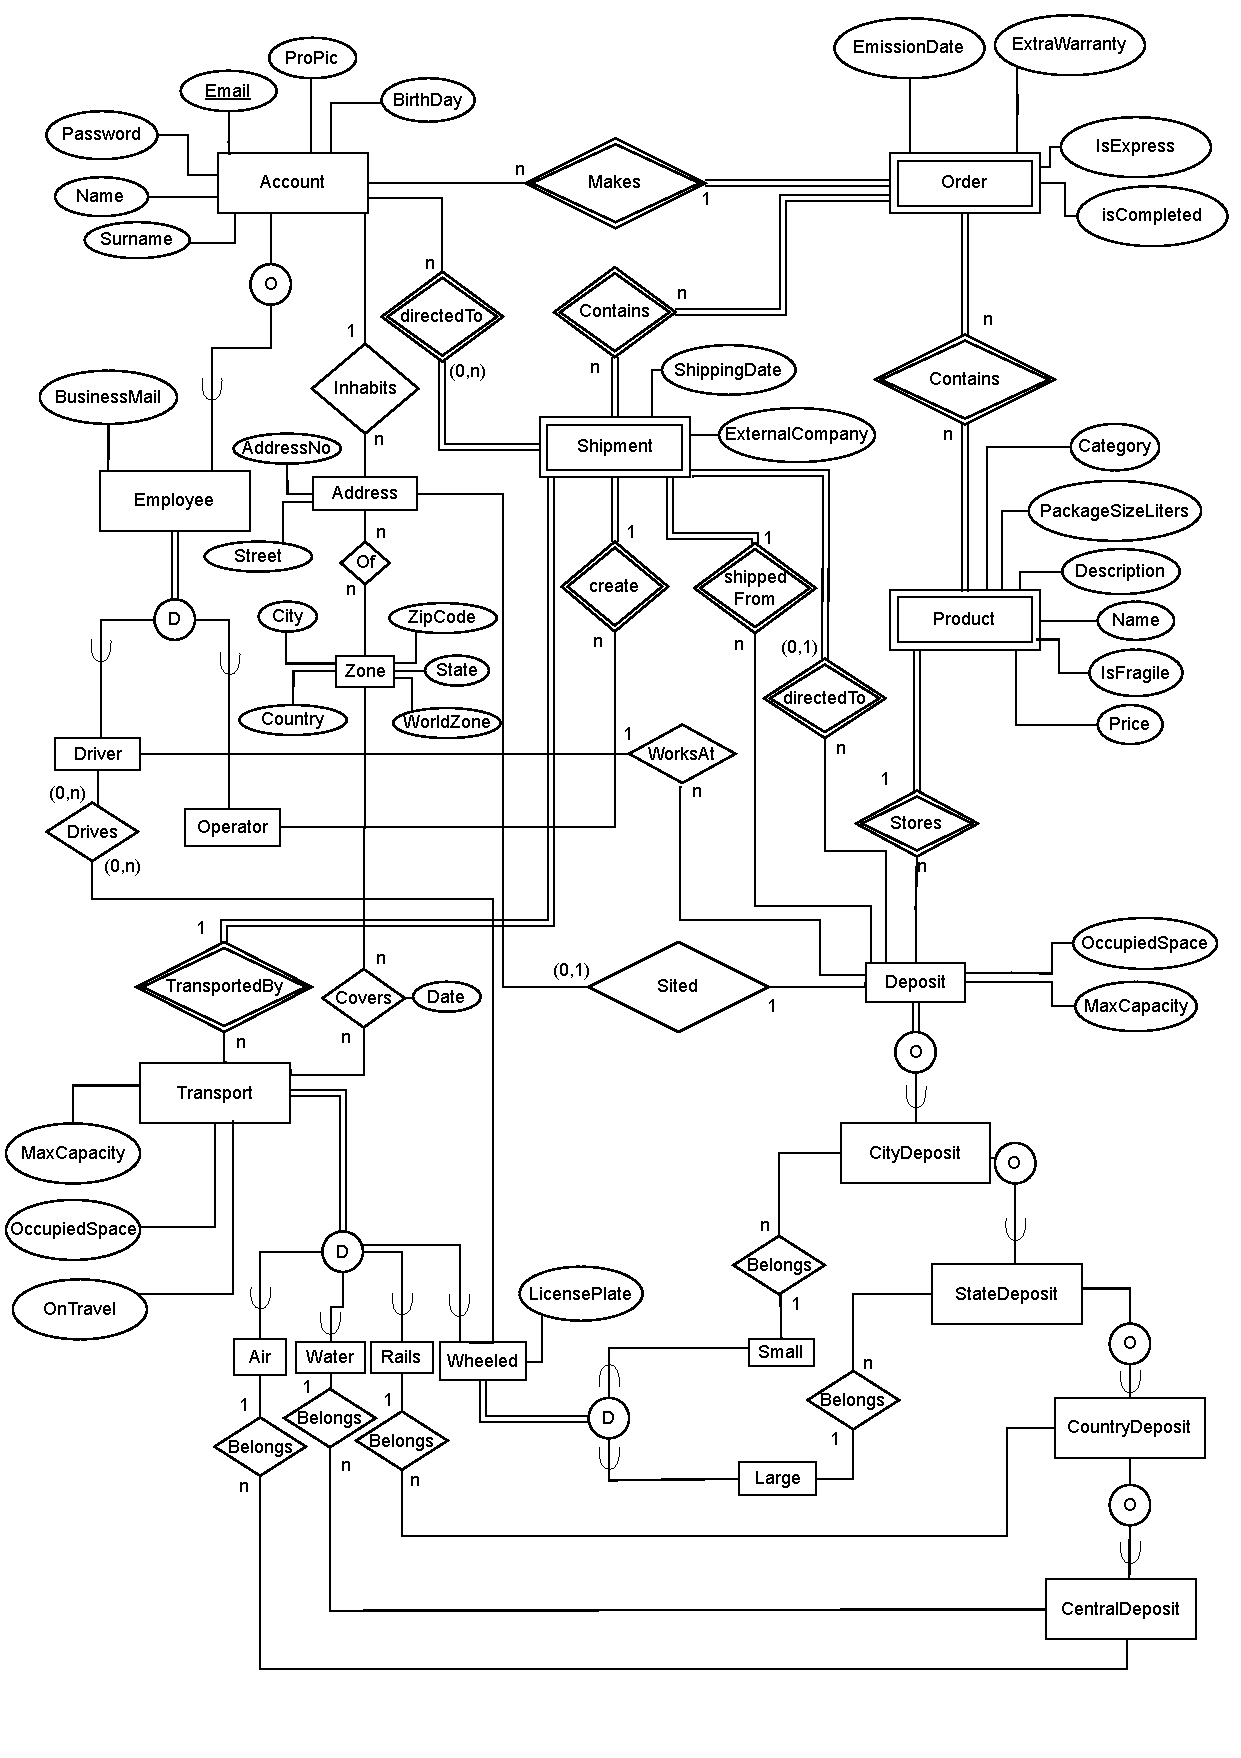
\includegraphics[width=0.9\textwidth]{ER_Diagram.pdf}
\end{center}

\section{UML Class Diagram}
\begin{center}
  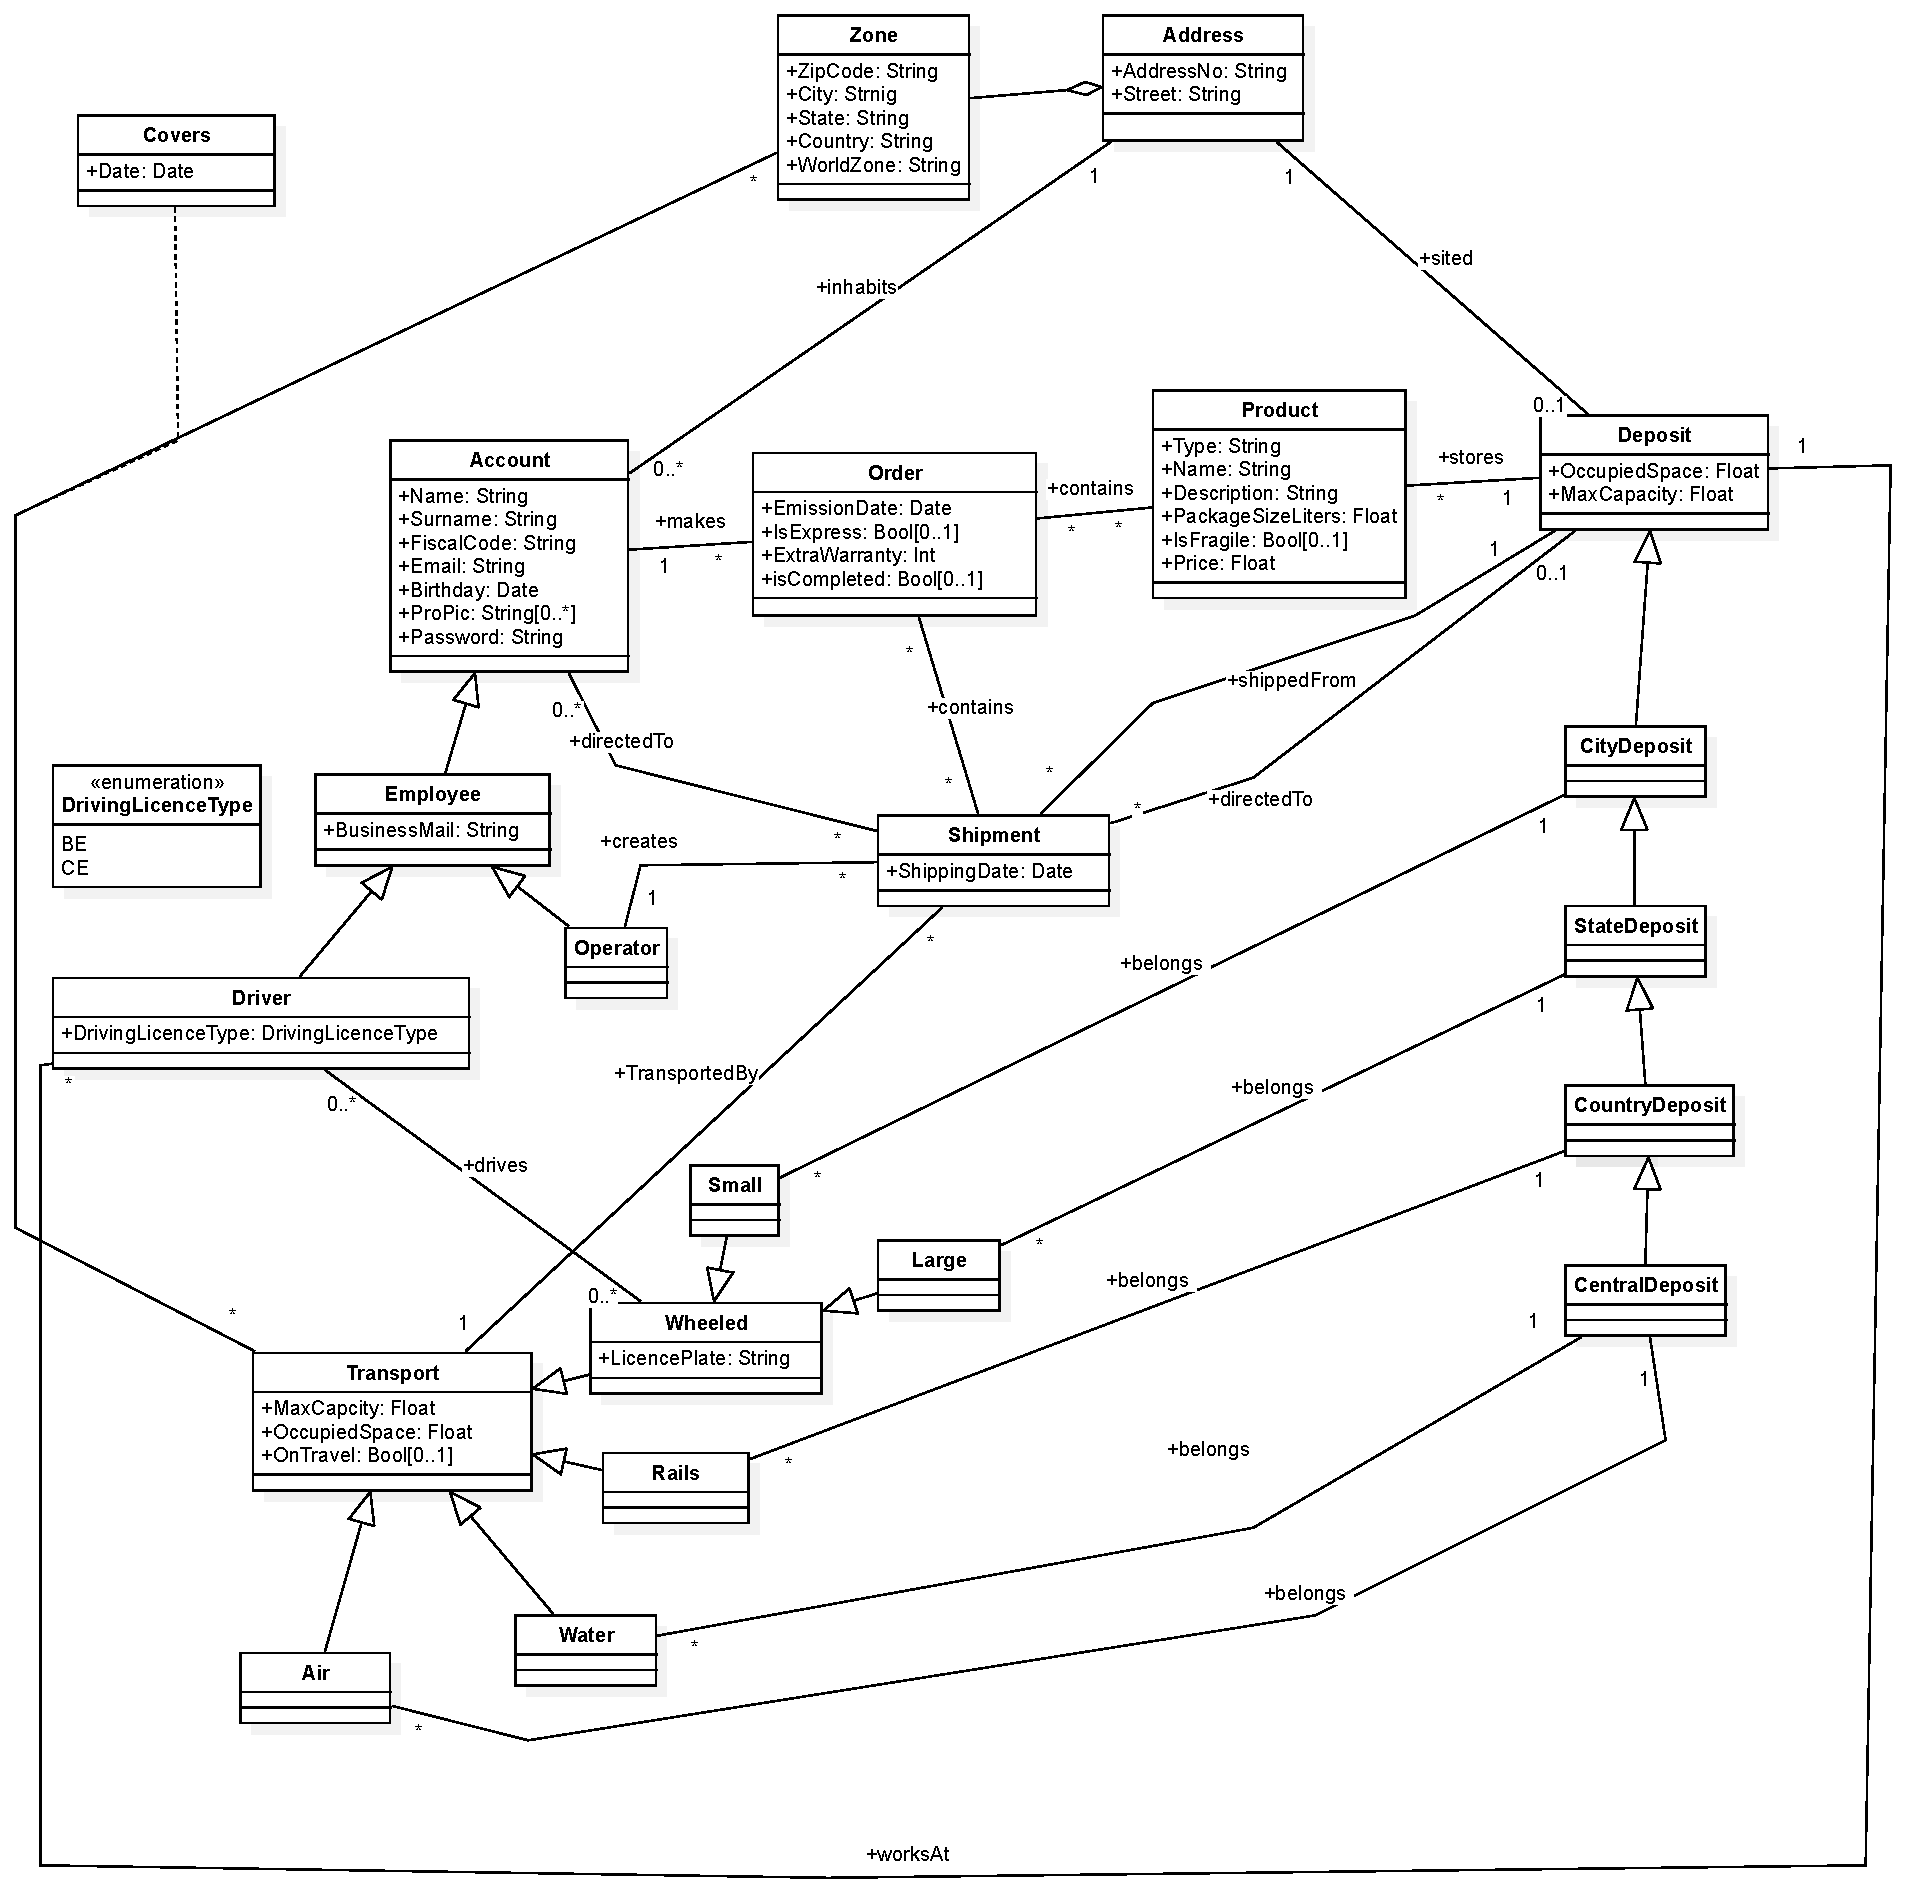
\includegraphics[width=\textwidth]{UML_Class_Diagram.pdf}
\end{center}

\section{Ristrutturazione del Diagramma UML}

% TODO: @RiccardoElena @zGenny write this section
  % it should contains:
  % 1) all the considerations about the UML diagram
  % 2) the changes made to the UML diagram
  % 3) the new UML diagram
  % 4) constrints dictonary (table (?)). Styled as the example in the slides